% Created by tikzDevice version 0.6.2-92-0ad2792 on 2013-01-11 06:31:19
% !TEX encoding = UTF-8 Unicode
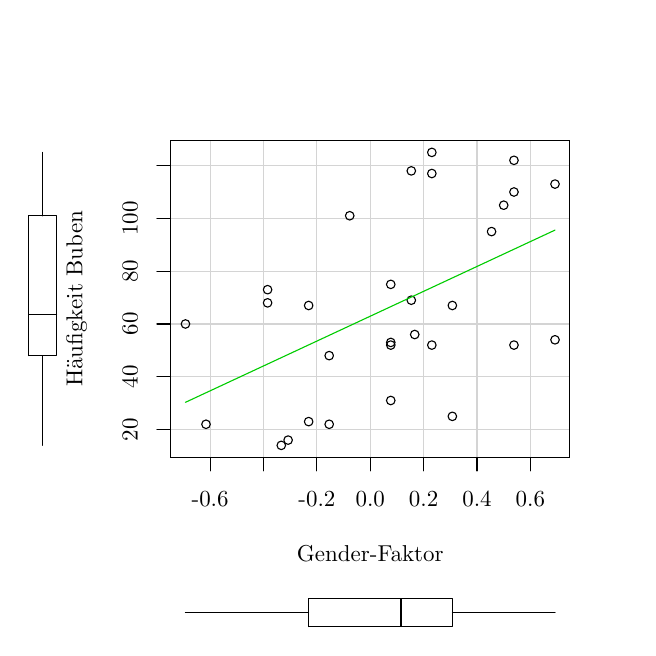
\begin{tikzpicture}[x=1pt,y=1pt]
\definecolor[named]{fillColor}{rgb}{1.00,1.00,1.00}
\path[use as bounding box,fill=fillColor,fill opacity=0.00] (0,0) rectangle (216.81,216.81);
\begin{scope}
\path[clip] (  0.00, 61.64) rectangle ( 10.84,175.97);
\definecolor[named]{drawColor}{rgb}{0.00,0.00,0.00}

\path[draw=drawColor,line width= 0.4pt,line join=round,line cap=round] (  0.40, 98.30) --
	( 10.44, 98.30) --
	( 10.44,148.85) --
	(  0.40,148.85) --
	(  0.40, 98.30);

\path[draw=drawColor,line width= 0.4pt,line join=round,line cap=round] (  0.40,113.08) --
	( 10.44,113.08);

\path[draw=drawColor,line width= 0.4pt,line join=round,line cap=round] (  5.42, 65.87) --
	(  5.42, 98.30);

\path[draw=drawColor,line width= 0.4pt,line join=round,line cap=round] (  5.42,148.85) --
	(  5.42,171.74);
\end{scope}
\begin{scope}
\path[clip] ( 51.68,  0.00) rectangle (195.89, 10.84);
\definecolor[named]{drawColor}{rgb}{0.00,0.00,0.00}

\path[draw=drawColor,line width= 0.4pt,line join=round,line cap=round] (101.53,  0.40) --
	(101.53, 10.44) --
	(153.46, 10.44) --
	(153.46,  0.40) --
	(101.53,  0.40);

\path[draw=drawColor,line width= 0.4pt,line join=round,line cap=round] (134.91,  0.40) --
	(134.91, 10.44);

\path[draw=drawColor,line width= 0.4pt,line join=round,line cap=round] ( 57.02,  5.42) --
	(101.53,  5.42);

\path[draw=drawColor,line width= 0.4pt,line join=round,line cap=round] (153.46,  5.42) --
	(190.55,  5.42);
\end{scope}
\begin{scope}
\path[clip] (  0.00,  0.00) rectangle (216.81,216.81);
\definecolor[named]{drawColor}{rgb}{0.00,0.00,0.00}

\path[draw=drawColor,line width= 0.4pt,line join=round,line cap=round] ( 65.92, 61.64) -- (181.65, 61.64);

\path[draw=drawColor,line width= 0.4pt,line join=round,line cap=round] ( 65.92, 61.64) -- ( 65.92, 56.66);

\path[draw=drawColor,line width= 0.4pt,line join=round,line cap=round] ( 85.21, 61.64) -- ( 85.21, 56.66);

\path[draw=drawColor,line width= 0.4pt,line join=round,line cap=round] (104.50, 61.64) -- (104.50, 56.66);

\path[draw=drawColor,line width= 0.4pt,line join=round,line cap=round] (123.79, 61.64) -- (123.79, 56.66);

\path[draw=drawColor,line width= 0.4pt,line join=round,line cap=round] (143.07, 61.64) -- (143.07, 56.66);

\path[draw=drawColor,line width= 0.4pt,line join=round,line cap=round] (162.36, 61.64) -- (162.36, 56.66);

\path[draw=drawColor,line width= 0.4pt,line join=round,line cap=round] (181.65, 61.64) -- (181.65, 56.66);

\node[text=drawColor,anchor=base,inner sep=0pt, outer sep=0pt, scale=  0.83] at ( 65.92, 43.71) {-0.6};

\node[text=drawColor,anchor=base,inner sep=0pt, outer sep=0pt, scale=  0.83] at (104.50, 43.71) {-0.2};

\node[text=drawColor,anchor=base,inner sep=0pt, outer sep=0pt, scale=  0.83] at (123.79, 43.71) {0.0};

\node[text=drawColor,anchor=base,inner sep=0pt, outer sep=0pt, scale=  0.83] at (143.07, 43.71) {0.2};

\node[text=drawColor,anchor=base,inner sep=0pt, outer sep=0pt, scale=  0.83] at (162.36, 43.71) {0.4};

\node[text=drawColor,anchor=base,inner sep=0pt, outer sep=0pt, scale=  0.83] at (181.65, 43.71) {0.6};

\path[draw=drawColor,line width= 0.4pt,line join=round,line cap=round] ( 51.68, 71.59) -- ( 51.68,166.97);

\path[draw=drawColor,line width= 0.4pt,line join=round,line cap=round] ( 51.68, 71.59) -- ( 46.70, 71.59);

\path[draw=drawColor,line width= 0.4pt,line join=round,line cap=round] ( 51.68, 90.67) -- ( 46.70, 90.67);

\path[draw=drawColor,line width= 0.4pt,line join=round,line cap=round] ( 51.68,109.74) -- ( 46.70,109.74);

\path[draw=drawColor,line width= 0.4pt,line join=round,line cap=round] ( 51.68,128.82) -- ( 46.70,128.82);

\path[draw=drawColor,line width= 0.4pt,line join=round,line cap=round] ( 51.68,147.90) -- ( 46.70,147.90);

\path[draw=drawColor,line width= 0.4pt,line join=round,line cap=round] ( 51.68,166.97) -- ( 46.70,166.97);

\node[text=drawColor,rotate= 90.00,anchor=base,inner sep=0pt, outer sep=0pt, scale=  0.83] at ( 39.72, 71.59) {20};

\node[text=drawColor,rotate= 90.00,anchor=base,inner sep=0pt, outer sep=0pt, scale=  0.83] at ( 39.72, 90.67) {40};

\node[text=drawColor,rotate= 90.00,anchor=base,inner sep=0pt, outer sep=0pt, scale=  0.83] at ( 39.72,109.74) {60};

\node[text=drawColor,rotate= 90.00,anchor=base,inner sep=0pt, outer sep=0pt, scale=  0.83] at ( 39.72,128.82) {80};

\node[text=drawColor,rotate= 90.00,anchor=base,inner sep=0pt, outer sep=0pt, scale=  0.83] at ( 39.72,147.90) {100};

\path[draw=drawColor,line width= 0.4pt,line join=round,line cap=round] ( 51.68, 61.64) --
	(195.89, 61.64) --
	(195.89,175.97) --
	( 51.68,175.97) --
	( 51.68, 61.64);
\end{scope}
\begin{scope}
\path[clip] ( 10.84, 10.84) rectangle (216.81,216.81);
\definecolor[named]{drawColor}{rgb}{0.00,0.00,0.00}

\node[text=drawColor,anchor=base,inner sep=0pt, outer sep=0pt, scale=  0.83] at (123.79, 23.79) {Gender-Faktor};

\node[text=drawColor,rotate= 90.00,anchor=base,inner sep=0pt, outer sep=0pt, scale=  0.83] at ( 19.80,118.81) {Häufigkeit Buben};
\end{scope}
\begin{scope}
\path[clip] ( 51.68, 61.64) rectangle (195.89,175.97);
\definecolor[named]{drawColor}{rgb}{0.83,0.83,0.83}

\path[draw=drawColor,line width= 0.4pt,line join=round,line cap=round] ( 65.92, 61.64) -- ( 65.92,175.97);

\path[draw=drawColor,line width= 0.4pt,line join=round,line cap=round] ( 85.21, 61.64) -- ( 85.21,175.97);

\path[draw=drawColor,line width= 0.4pt,line join=round,line cap=round] (104.50, 61.64) -- (104.50,175.97);

\path[draw=drawColor,line width= 0.4pt,line join=round,line cap=round] (123.79, 61.64) -- (123.79,175.97);

\path[draw=drawColor,line width= 0.4pt,line join=round,line cap=round] (143.07, 61.64) -- (143.07,175.97);

\path[draw=drawColor,line width= 0.4pt,line join=round,line cap=round] (162.36, 61.64) -- (162.36,175.97);

\path[draw=drawColor,line width= 0.4pt,line join=round,line cap=round] (181.65, 61.64) -- (181.65,175.97);

\path[draw=drawColor,line width= 0.4pt,line join=round,line cap=round] ( 51.68, 71.59) -- (195.89, 71.59);

\path[draw=drawColor,line width= 0.4pt,line join=round,line cap=round] ( 51.68, 90.67) -- (195.89, 90.67);

\path[draw=drawColor,line width= 0.4pt,line join=round,line cap=round] ( 51.68,109.74) -- (195.89,109.74);

\path[draw=drawColor,line width= 0.4pt,line join=round,line cap=round] ( 51.68,128.82) -- (195.89,128.82);

\path[draw=drawColor,line width= 0.4pt,line join=round,line cap=round] ( 51.68,147.90) -- (195.89,147.90);

\path[draw=drawColor,line width= 0.4pt,line join=round,line cap=round] ( 51.68,166.97) -- (195.89,166.97);
\end{scope}
\begin{scope}
\path[clip] (  0.00,  0.00) rectangle (216.81,216.81);
\definecolor[named]{drawColor}{rgb}{0.00,0.00,0.00}

\path[draw=drawColor,line width= 0.4pt,line join=round,line cap=round] ( 51.68, 61.64) --
	(195.89, 61.64) --
	(195.89,175.97) --
	( 51.68,175.97) --
	( 51.68, 61.64);
\end{scope}
\begin{scope}
\path[clip] ( 51.68, 61.64) rectangle (195.89,175.97);
\definecolor[named]{drawColor}{rgb}{0.00,0.00,0.00}

\path[draw=drawColor,line width= 0.4pt,line join=round,line cap=round] (131.20,102.11) circle (  1.55);

\path[draw=drawColor,line width= 0.4pt,line join=round,line cap=round] (108.95, 73.50) circle (  1.55);

\path[draw=drawColor,line width= 0.4pt,line join=round,line cap=round] (108.95, 98.30) circle (  1.55);

\path[draw=drawColor,line width= 0.4pt,line join=round,line cap=round] (138.62,165.06) circle (  1.55);

\path[draw=drawColor,line width= 0.4pt,line join=round,line cap=round] (138.62,118.33) circle (  1.55);

\path[draw=drawColor,line width= 0.4pt,line join=round,line cap=round] (153.46,116.42) circle (  1.55);

\path[draw=drawColor,line width= 0.4pt,line join=round,line cap=round] (172.01,152.66) circle (  1.55);

\path[draw=drawColor,line width= 0.4pt,line join=round,line cap=round] ( 91.64, 65.87) circle (  1.55);

\path[draw=drawColor,line width= 0.4pt,line join=round,line cap=round] (131.20,103.07) circle (  1.55);

\path[draw=drawColor,line width= 0.4pt,line join=round,line cap=round] ( 64.44, 73.50) circle (  1.55);

\path[draw=drawColor,line width= 0.4pt,line join=round,line cap=round] (131.20,124.05) circle (  1.55);

\path[draw=drawColor,line width= 0.4pt,line join=round,line cap=round] ( 94.11, 67.78) circle (  1.55);

\path[draw=drawColor,line width= 0.4pt,line join=round,line cap=round] (153.46, 76.36) circle (  1.55);

\path[draw=drawColor,line width= 0.4pt,line join=round,line cap=round] (175.72,102.11) circle (  1.55);

\path[draw=drawColor,line width= 0.4pt,line join=round,line cap=round] (139.86,105.93) circle (  1.55);

\path[draw=drawColor,line width= 0.4pt,line join=round,line cap=round] (101.53, 74.46) circle (  1.55);

\path[draw=drawColor,line width= 0.4pt,line join=round,line cap=round] (131.20, 82.09) circle (  1.55);

\path[draw=drawColor,line width= 0.4pt,line join=round,line cap=round] (116.37,148.85) circle (  1.55);

\path[draw=drawColor,line width= 0.4pt,line join=round,line cap=round] (146.04,102.11) circle (  1.55);

\path[draw=drawColor,line width= 0.4pt,line join=round,line cap=round] ( 86.69,117.37) circle (  1.55);

\path[draw=drawColor,line width= 0.4pt,line join=round,line cap=round] (190.55,160.29) circle (  1.55);

\path[draw=drawColor,line width= 0.4pt,line join=round,line cap=round] ( 86.69,122.14) circle (  1.55);

\path[draw=drawColor,line width= 0.4pt,line join=round,line cap=round] (175.72,157.43) circle (  1.55);

\path[draw=drawColor,line width= 0.4pt,line join=round,line cap=round] ( 57.02,109.74) circle (  1.55);

\path[draw=drawColor,line width= 0.4pt,line join=round,line cap=round] (146.04,171.74) circle (  1.55);

\path[draw=drawColor,line width= 0.4pt,line join=round,line cap=round] (175.72,168.88) circle (  1.55);

\path[draw=drawColor,line width= 0.4pt,line join=round,line cap=round] (146.04,164.11) circle (  1.55);

\path[draw=drawColor,line width= 0.4pt,line join=round,line cap=round] (190.55,104.02) circle (  1.55);

\path[draw=drawColor,line width= 0.4pt,line join=round,line cap=round] (167.62,143.13) circle (  1.55);

\path[draw=drawColor,line width= 0.4pt,line join=round,line cap=round] (101.53,116.42) circle (  1.55);
\definecolor[named]{drawColor}{rgb}{0.00,0.80,0.00}

\path[draw=drawColor,line width= 0.4pt,line join=round,line cap=round] ( 57.02, 81.43) --
	(190.55,143.66);
\end{scope}
\end{tikzpicture}
